\section{Properties Of The Clay 黏土的物理特性}

\begin{paracol}{2}

    The clay used for this study is a normally consolidated marine clay located at a place called Skabo, 2 miles west from the centre of Oslo. The undisturbed samples were obtained by the Norwegian Geotechnical Institute's thin-walled stationary piston sampler recovering samples of 80 cm long and 54 mm dia. In order to ensure homogeneity of the material used for the testing, the samples were taken from the same depths, 15-16 m, in eight boreholes made in the same vicinity.

    \switchcolumn

    这项研究使用的黏土是一种普通固结的海洋黏土,位于奥斯陆市中心以西2英里处的Skabo。 不受干扰的样品是由挪威地质技术研究所的薄壁固定式活塞取样器获得的,回收的样品长80厘米,直径54毫米。 为了确保试验所用材料的均匀性,从15-16m的相同深度的样品中,在附近进行了八个钻孔。

\end{paracol}

\begin{table*}[!htb]
    \centering
    \caption{Properties of Skabo clay}
    \addtocounter{table}{-1}
    \vspace{-8pt}
    \renewcommand{\tablename}{表}
    \caption{Skabo黏土的物理特性}
    \vspace{4pt}
    \renewcommand{\tablename}{Table}
    \begin{tabular}{ll|ll}
        \Xhline{1pt}
        Properties & value & Properties & value \\
        \Xcline{1-4}{0.7pt}
        Water content, $\%$ & 43.1 (39.4-47.8) & Activity & 0.63 \\
        Liquid limit & 52 & Salt content, g/L & 25 (24.2-28.8) \\
        Plastic limit & 24 & Organic content, $\%$ & 0.32 \\
        Plastic index  & 28 & $S_u/p$ & 0.25 \\
        Clay fraction $<2\mu ,\%$ & 45 & Sensitivity & 5\\
        \Xhline{1pt}
    \end{tabular}%
    \label{table:1}%
\end{table*}


\begin{paracol}{2}

    The results of the standard field and laboratory tests carried out at Skabo are summarized in \autoref{figure:1}. The data of the clay used in the present programme are summarized in \autoref{table:1}.

    \switchcolumn
        
    Skabo进行的标准现场试验和实验室试验的结果总结在\cnfigureref{figure:1}中。本程序中使用的黏土的数据总结在\cntableref{table:1}中。

    \switchcolumn*

    The clay used for this study is a normally consolidated marine clay located at a place called Skabo, 2 miles west from the centre of Oslo. The undisturbed samples were obtained by the Norwegian Geotechnical Institute's thin-walled stationary piston sampler recovering samples of 80 cm long and 54 mm dia. In order to ensure homogeneity of the material used for the testing, the samples were taken from the same depths, 15-16 m, in eight boreholes made in the same vicinity.

    \switchcolumn      
    
    这项研究使用的黏土是一种普通固结的海洋黏土,位于奥斯陆市中心以西2英里处的Skabo。 不受干扰的样品是由挪威地质技术研究所的薄壁固定式活塞取样器获得的,回收的样品长80厘米,直径54毫米。 为了确保试验所用材料的均匀性,从15-16m的相同深度的样品中,在附近进行了八个钻孔。

    \switchcolumn*      
    
    The results of the standard field and laboratory tests carried out at Skabo are summarized in \autoref{figure:1}. The data of the clay used in the present programme are summarized in \autoref{table:1}.

    \switchcolumn              
    
    Skabo进行的标准现场试验和实验室试验的结果总结在\cnfigureref{figure:1}中。本程序中使用的黏土的数据总结在\cntableref{table:1}中。
    \switchcolumn*
    
\end{paracol}

\begin{figure}[!h]
    \centering
    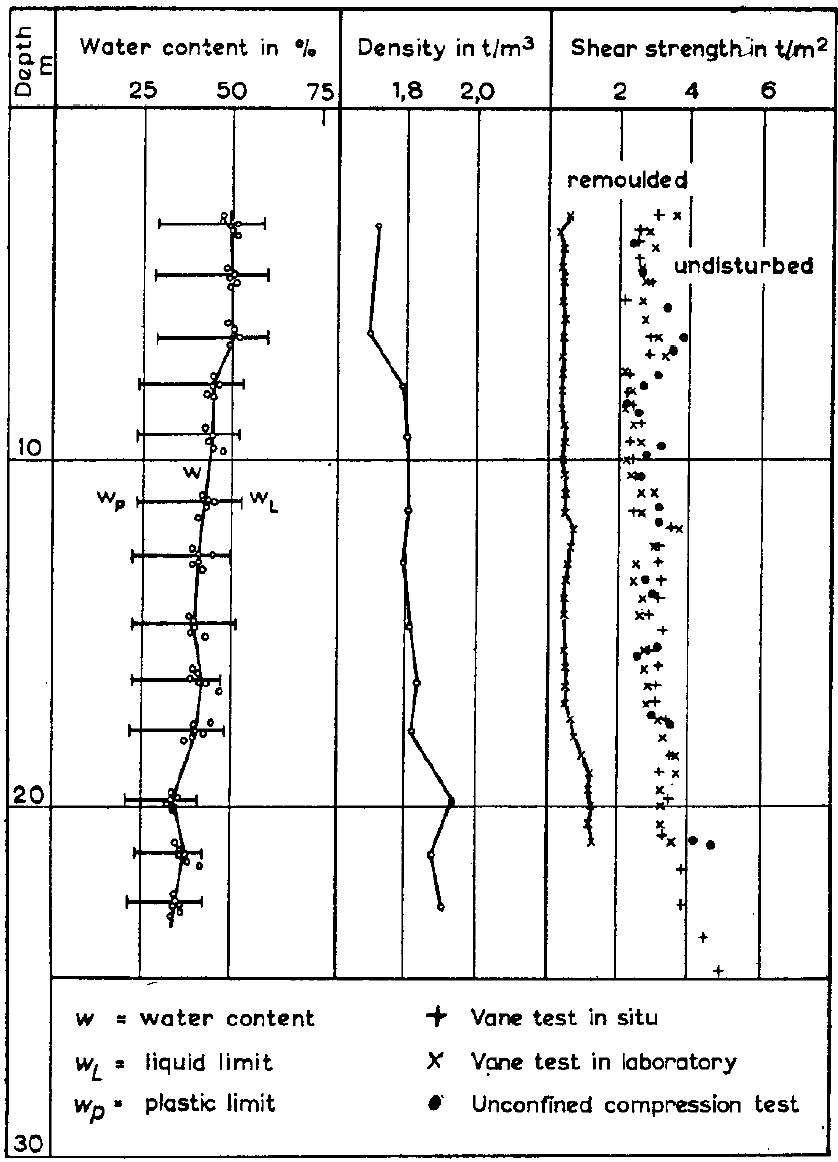
\includegraphics[width=0.5\textwidth]{figures/figure-1.png}
    \caption{Geotechnical profile through Skabo clay with results of field and laboratory tests}
    \addtocounter{figure}{-1}
    \vspace{-5pt}
    \renewcommand{\figurename}{图}
    \caption{通过Skabo黏土进行的岩土工程剖面以及现场和实验室试验的结果}
    \renewcommand{\figurename}{Figure}
    \label{figure:1}
\end{figure}


\begin{paracol}{2}

    \noindent From the boring records in \autoref{figure:1} it is seen directly that the clay, is unusually homogeneous with approximately constant Atterberg limits and water content between the depths of 8 and 18 m. 

    \switchcolumn

    \noindent 从\cnfigureref{figure:1}的记录中可以直接看到,黏土异常均匀,具有近似恒定的阿特伯格极限,并且水深在8至18 m之间。

    \switchcolumn*

    Results of X-ray examination and differential thermal analysis showed that the clay fraction was composed of about 40$\%$ illite, 20$\%$ chlorite, 25$\%$ quartz, and 15$\%$ feldspar. Except for the presence of the appreciable amount of chlorite, the mineralogical composition may be considered as typically representative of the clay in the Oslo region.

    \switchcolumn

    X射线检查和差热分析的结果表明,黏土部分由约40$\%$的伊利石,20$\%$的绿泥石,25$\%$的石英和15$\%$的长石组成。 除了存在可观数量的亚氯酸盐外,矿物​​学组成通常被认为是奥斯陆地区黏土的典型代表。

    \switchcolumn*

    The results of about forty consolidation tests showed that the soil has a "weathered" zone approximately 11 m thick and below this depth the deposit is normally consolidated. This finding is confirmed by a study of the variation in undrained shear strength with depth. Below a depth of about 11 m the clay exhibits a linear increase of shear strength with depth. The ratio of the undrained shear strength to the consolidation pressure is 0·25 for the layer considered. The undrained shear strength being determined in situ by vane tests and in the laboratory by vane tests and unconfined compression tests.

    \switchcolumn
        
    大约四十次固结试验的结果表明,土壤具有大约11 m厚的“风化”区,在该深度以下,沉积物通常被固结。 通过研究不排水抗剪强度随深度的变化,证实了这一发现。 在约11 m的深度以下,黏土的剪切强度随深度呈线性增加。 对于所考虑的层,不排水的剪切强度与固结压力之比为0.25。 不排水的剪切强度是通过现场十字板剪切试验确定的,而在实验室中是通过十字板剪切试验和无侧限压缩试验确定的。

    \switchcolumn*

    All samples tested were undisturbed but reconsolidated at a pressure well above the effect stresses which the samples carried in the field, so that they can be considered as normally consolidated.

    \switchcolumn
        
    所有试验的样品均未受干扰,但在远高于样品在野外所承受的作用应力的压力下重新固结,因此可以将其视为正常固结。
    
\end{paracol}